% ch2p22_001: Pics: The Angle revisited
\documentclass[tikz, border=10pt]{standalone}

\usepackage{tikz}
\usetikzlibrary{angles, quotes}

\begin{document}
	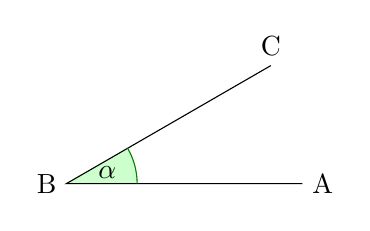
\begin{tikzpicture}[scale=3]
		\coordinate (A) at (1, 0);
		\coordinate (B) at (0, 0);
		\coordinate (C) at (30:1cm);
		
		\draw (A) node[right] {A} -- (B) node[left] {B} -- (C) node[above] {C}
			pic[draw=green!50!black, fill=green!20, angle radius=9mm, "$\alpha$"] {angle = A--B--C};
	\end{tikzpicture}
\end{document}